\begin{refsection}

\chapter{\textit{TBX1} gene mutation screening in non-syndromic CTHD} % Main chapter title
\chaptermark{\normalfont \textit{TBX1} gene mutation screening}
\label{Chapter4} % Change X to a consecutive number; for referencing this chapter elsewhere, use \ref{ChapterX}

%----------------------------------------------------------------------------------------
%	SECTION 1
%----------------------------------------------------------------------------------------

\section{Introduction}
Molecular evaluation of genetic syndromes with CTHD has provided valuable insight into their genetic basis. In particular, studies on the 22q11.2 microdeletion syndrome defined a large CTHD population and identified genes and developmental pathways contributing to cardiac development and disease. The 22q11.2 deletion, which is mediated by non-homologous recombination between low copy repeats, typically removes a genomic segment including the cardiac transcription factor \textit{TBX1}. 

\textit{TBX1} is a member of a phylogenetically conserved family of genes that share a common DNA-binding domain, the T-box. T-box genes are transcription factors involved in the regulation of key developmental processes. Mouse \textit{Tbx1} has previously shown to be expressed during early embryogenesis in the pharyngeal arches, pouches, and optic vesicle. Later in development, expression is seen in the vertebral column and tooth bud. Jerome and Papaioannou \cite{jerome2001digeorge} studied the mouse gene encoding the \textit{Tbx1} transcription factor in a genetically engineered haploinsufficient (\textit{Tbx1}-/+) or null (\textit{Tbx1}-/-) mice. \textit{Tbx1}-/- mice died in utero with abnormal facies and thymus and parathyroid aplasia along with heart failure and malformed cardiac outflow tracts and aortic arches. Although \textit{Tbx1}-/+ mice were viable and had no non-cardiovascular abnormalities, many had like aortic arch abnormalities.

Aortic arch abnormalities were also observed by Lindsay et al \cite{lindsay1999congenital, lindsay2001tbx1} and Merscher et al \cite{merscher2001tbx1}, who independently created mice hemizygous for large genomic segments including \textit{Tbx1} and other genes. Both groups showed that specific replacement of only the \textit{Tbx1} gene corrected aortic defects. These findings are taken as evidence that even human CTHD can be caused by alterations in gene dose of \textit{TBX1}. 

Human studies have identified nine novel variants of \textit{TBX1} that alter protein sequence in cases who have the phenotype of the 22q11.2 microdeletion, including CTHD, but who do not carry the chromosomal microdeletion \cite{gong2001mutation, lindsay2001tbx1}. Some of these mutations completely ablate \textit{TBX1} function in vitro, while others result in a gain of \textit{TBX1} function, suggesting an optimal range of \textit{TBX1} activity above or below which the risk of malformations increases. 

The suggested role of \textit{TBX1} in cardiac development - supported with mouse models showing developmental defects attributable to \textit{Tbx1} only - have set the basis of the design for this part of the study. The hypothesis is that hypomorphic alleles of \textit{TBX1} which reduce but do not completely ablate \textit{TBX1} function, might be involved in susceptibility to non-syndromic CTHD. Exons 4, 5, 6, and 7 of \textit{TBX1} are located in T-box region and show 98\% homology to mouse \textit{Tbx1}. Therefore, to clarify the role and to detect any possible causative relation of \textit{TBX1} mutations in CTHD, the study was extended to this homology region. Also, an attempt was made to establish the most frequent heart defects in both groups to determine selection criteria for at risk patients in our population

\section{Methodology}
DNA was isolated from the blood of the 96 cases and 100 controls as detailed in Section 2.3.3 Mutations or variations in exons 4, 5, 5, 6, 7 of \textit{TBX1} were analyzed by PCR with sequence specific primers (\cref{tab:4.1primers}) Due to their lengths, exon 5 and exon 6 were amplified  with two sets of primers PCR amplifications were performed following an initial denaturation at 95 ºC for 5 min, 95 ºC  for  30 s, Tm for 1 min for 30 cycles  followed by a final extension for 10 min at 72 ºC. After a quality check in a 2\% agarose gel, the amplicons were processed for Sanger sequencing as outlined in section 2.3.7. The sequences obtained were aligned with the reference sequence using the SeqScape analysis software V2.5 and analyzed for sequence variants.

\begin{table}[!thbp]
\centering
\caption{PCR primers and reaction conditions used to amplify selected \textit{TBX1} exons \cite{Cabuk2007}}
\label{tab:4.1primers}
\begin{tabular}{  l  l  l  l  }
\toprule
	\textbf{Exon} & \textbf{Amplicon size} & \textbf{Tm (ºC)} & \textbf{Primer sequence} \\ \toprule
	4 & 178 & 55ºC & F:5’ TGC CTT CCA CCA GCT AGG 3’ \\ 
	 &  &  & R:5’CCG GTC CCT CAC GCT TAC 3’ \\ \midrule
	5A & 194 & 60 ºC & F:5’CTC GGG TTC ACC TCC ACA T \\ 
	 &  &  & R:5’CAG CTT GAG CTT GTC GAA GG 3’ \\ \midrule
	5B & 179 & 60 ºC & F:5’CGG ACT CGC CTG CCA AGG 3’ \\ 
	 &  &  & R:5’CAG GCC TCT TAG GGA CAG G 3’ \\ \midrule
	6A & 197 & 60 ºC & F:5’CTC CCA CCC CAC ATC CTC \\ 
	 &  &  & R:5’CCG CGG TGA ATC GTG TCT C 3’ \\ \midrule
	6B & 175 & 60 ºC & F:5’TCC ATG CAC AGA TAC CAG C3’ \\ 
	 &  &  & R:5’AAT CCG CTC AGG TCC AGC 3’ \\ \midrule
	7 & 149 & 65 & F:5’AGG CTG CAG GGC TCC AGC 3’ \\ 
	 &  &  & R:5’CGC CCG GCG CTC ACT CTC 3’ \\ \bottomrule
\end{tabular}
\end{table}

\section{Results}
The most frequent type of CTHD observed in both groups was TOF as shown in \cref{fig:4_2,fig:4_3}. Among the study subjects, no pathogenic mutations or sequence variants were detected (\cref{fig:4_4,fig:4_5,fig:4_6,fig:4_7,fig:4_8,fig:4_9}). Seventy three were isolated CTHD and the 23 cases had at least one extra-cardiac phenotype of the 22q11 microdeletion. The extra-cardiac features recorded included facial dysmorphism (74\%), mild intellectual disability (91\%) and thymic or parathyroid gland hypoplasia/aplasia (4\%). 

%\begin{figure}[!thbp]
%\centering
%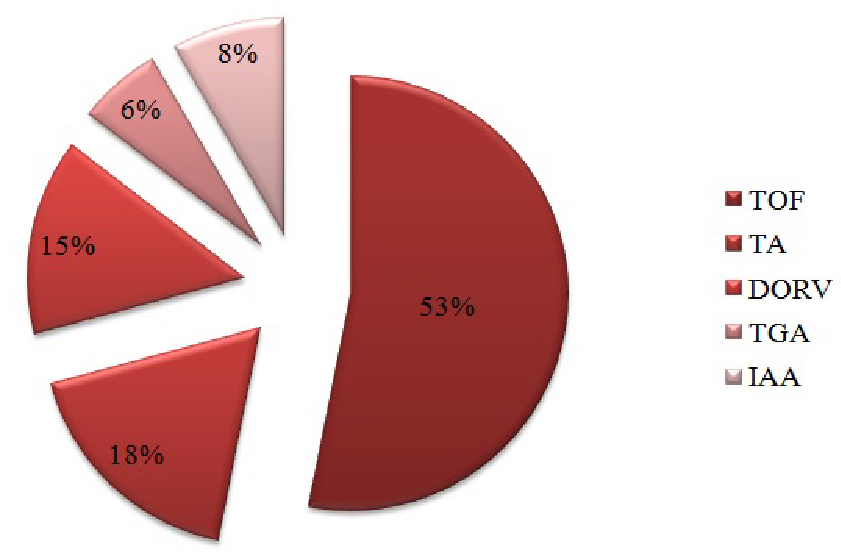
\includegraphics[width=\linewidth]{Figures/Figure4_1pie.pdf}
%\rule{35em}{0.5pt}
%\caption{Distribution of CTHD in the studied case population %(n=96)}
%\label{fig:4_1}
%\end{figure}

\begin{figure}[!thbp]
\centering
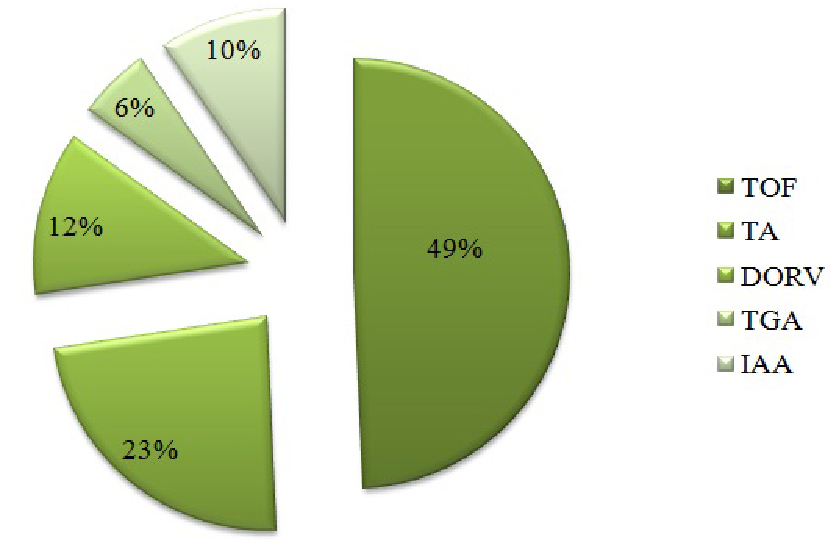
\includegraphics[scale=0.65,keepaspectratio]{Figures/Figure4_2pie.pdf}
\rule{35em}{0.5pt}
\caption{Distribution of isolated CTHD in the studied case population (n=73)}
\label{fig:4_2}
\end{figure}

\begin{figure}[!thbp]
\centering
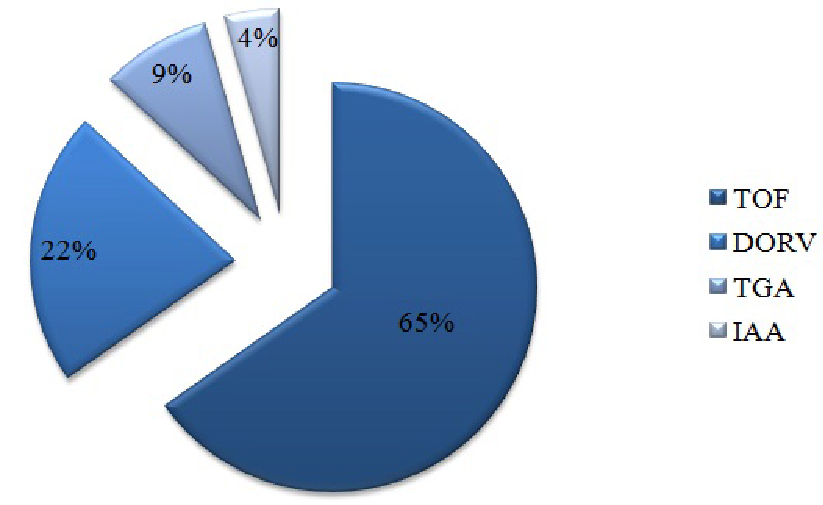
\includegraphics[scale=0.65]{Figures/Figure4_3pie.pdf}
\rule{35em}{0.5pt}
\caption{Distribution of CTHD with at least one extra-cardiac feature (n=23)}
\label{fig:4_3}
\end{figure}

\begin{figure}[!thbp]
\centering
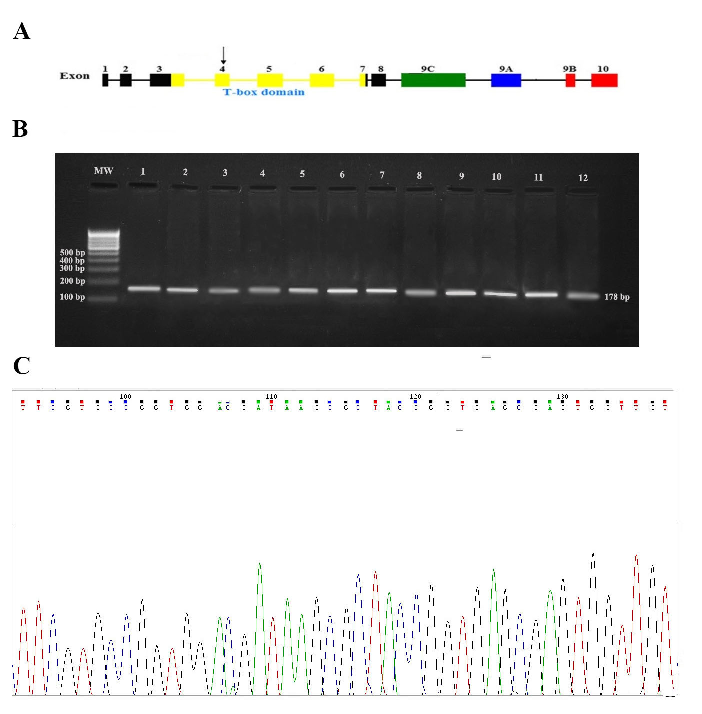
\includegraphics[width=\linewidth]{Figures/Figure4_4TBX4.pdf}
\rule{35em}{0.5pt}
\caption{\textbf{The screening results of the \textit{TBX1} exon 4 coding sequence.}
\textbf{A.} Schematic representation of \textit{TBX1} indicating the position of exon 4 in the T domain 
\textbf{B.} 2\% agarose gel showing the amplicon of representative cases with size 178 bp 
\textbf{C.} Representative electropherogram (case \#69) of exon 4}
\label{fig:4_4}
\end{figure}

\begin{figure}[!thbp]
\centering
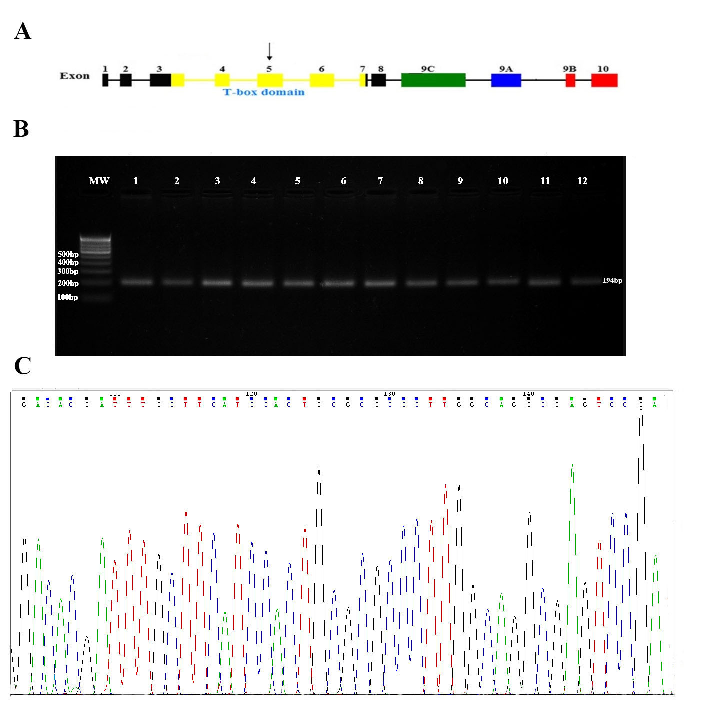
\includegraphics[width=\linewidth]{Figures/Figure4_5TBX5A.pdf}
\rule{35em}{0.5pt}
\caption{\textbf{The screening results of the \textit{TBX1} exon 5A coding sequence.}
\textbf{A.} Schematic representation of \textit{TBX1} indicating the position of exon 5A in the T domain 
\textbf{B.} 2\% agarose gel showing the amplicon of representative cases with size 194 bp \textbf{C.} Representative electropherogram (case \#63) of exon 5A}
\label{fig:4_5}
\end{figure}

\begin{figure}[!thbp]
\centering
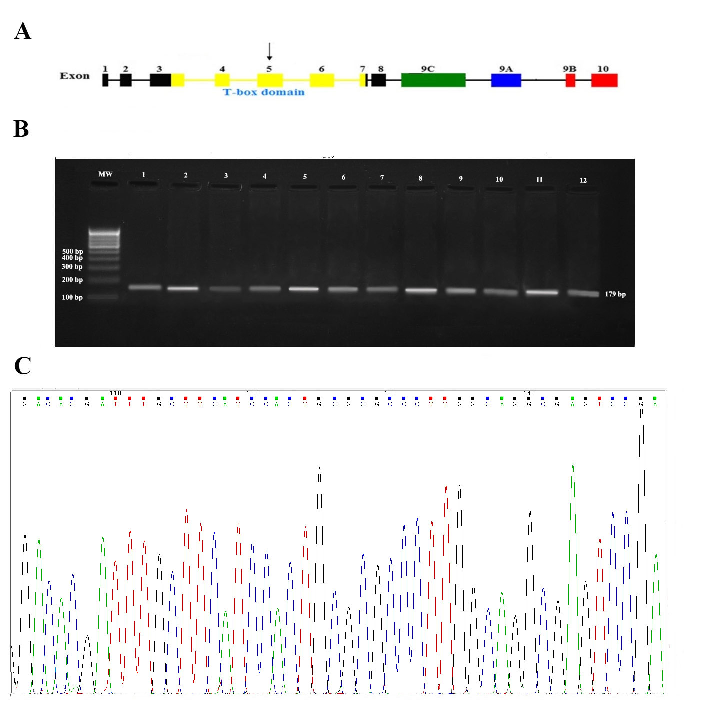
\includegraphics[width=\linewidth]{Figures/Figure4_6TBX5B.pdf}
\rule{35em}{0.5pt}
\caption{\textbf{The screening results of the \textit{TBX1} exon 5B coding sequence.}
\textbf{A.} Schematic representation of \textit{TBX1} indicating the position of exon 5B in the T domain \textbf{B.} 2\% agarose gel showing the amplicon of representative cases with size 179 bp \textbf{C.} Representative electropherogram (case \#43) of exon 5B}
\label{fig:4_6}
\end{figure}


\begin{figure}[!thbp]
\centering
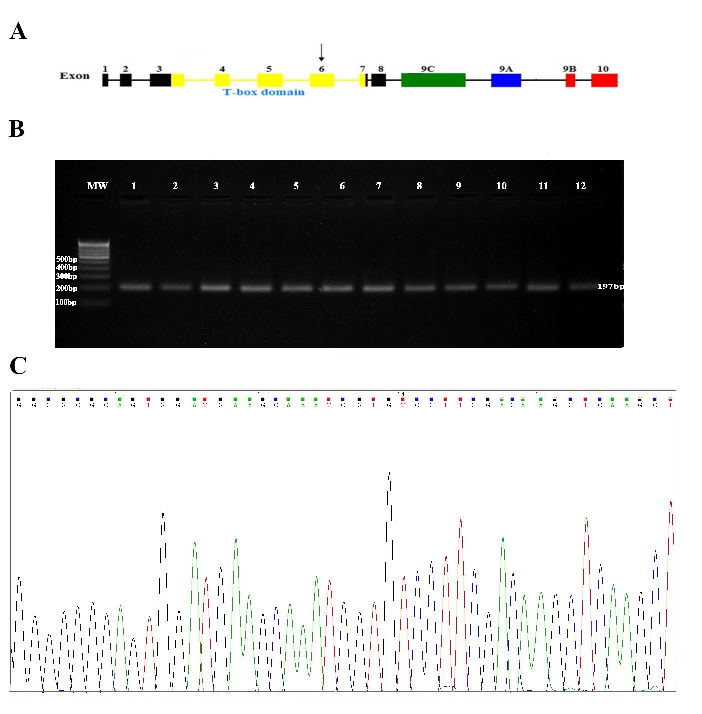
\includegraphics[width=\linewidth]{Figures/Figure4_7TBX6A.pdf}
\rule{35em}{0.5pt}
\caption{\textbf{The screening results of the \textit{TBX1} exon 6A coding sequence.}
\textbf{A.} Schematic representation of \textit{TBX1} indicating the position of exon 6A in the T domain \textbf{B.} 2\% agarose gel showing the amplicon of representative cases with size 197 bp \textbf{C.} Representative electropherogram (case \#15) of exon 6A}
\label{fig:4_7}
\end{figure}


\begin{figure}[!thbp]
\centering
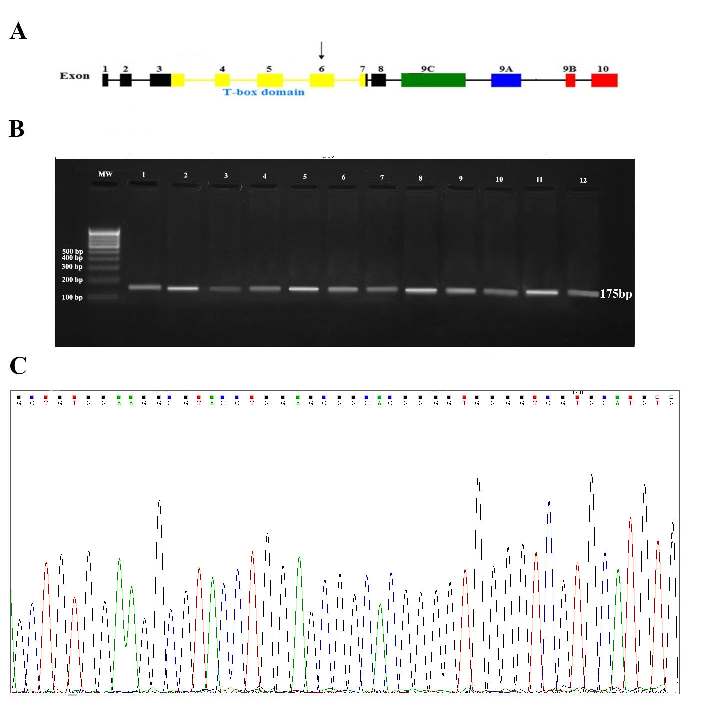
\includegraphics[width=\linewidth]{Figures/Figure4_8TBX6B.pdf}
\rule{35em}{0.5pt}
\caption{\textbf{The screening results of the \textit{TBX1} exon 6B coding sequence.}
\textbf{A.} Schematic representation of \textit{TBX1} indicating the position of exon 6B in the T domain \textbf{B.} 2\% agarose gel showing the amplicon of representative cases with size 175 bp \textbf{C.} Representative electropherogram (case \#15) of exon 6B}
\label{fig:4_8}
\end{figure}

\begin{figure}[!thbp]
\centering
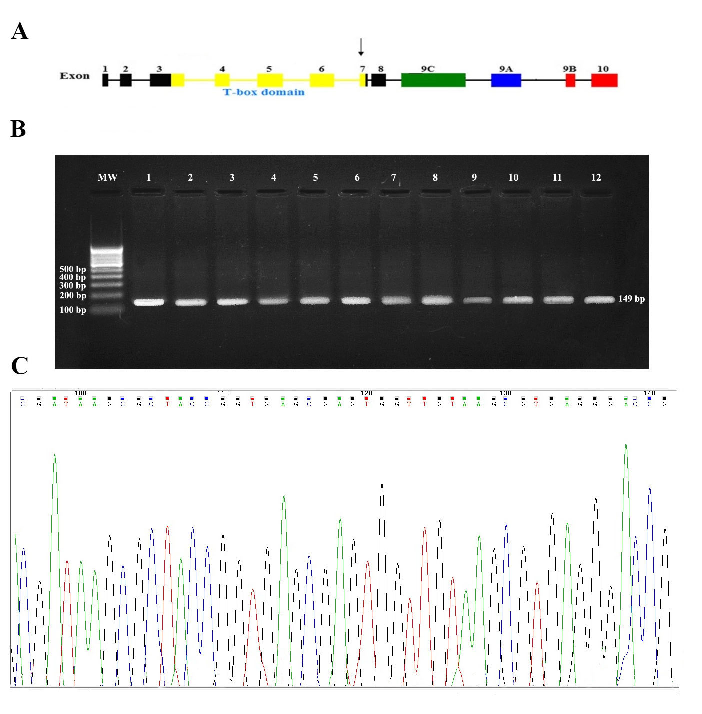
\includegraphics[width=\linewidth]{Figures/Figure4_9TBX7.pdf}
\rule{35em}{0.5pt}
\caption{\textbf{The screening results of the \textit{TBX1} exon 7 coding sequence.}
\textbf{A.} Schematic representation of the \textit{TBX1} gene. indicating the position of exon 7 in the T domain \textbf{B.} 2\% agarose gel showing the amplicon of representative cases with size 149 bp \textbf{C.} Representative electropherogram (case \#36) of exon 7}
\label{fig:4_9}
\end{figure}



\section{Discussion}


\textit{TBX1} is thought to be a major candidate gene that influences the cardiac phenotype or its severity in patients carrying the 22q11.2 deletion \cite{gong2001mutation}. Its dose dependent role in heart development has been demonstrated in mouse models \cite{chieffo1997isolation, lindsay1999congenital, lindsay2001tbx1}. Therefore, screening of the \textit{TBX1} gene would likely indicate whether the sequence variants or mutations would have an impact on cardiac phenotype. However, no mutation or previously reported polymorphism was observed in both the cases with isolated CTHD as well as CTHD with extra-cardiac findings. Considering the strong experimental evidence for a major role of \textit{Tbx1} in CTHD from the deletion studies in the mouse (1, 4, 9) these results are somewhat surprising. It is likely that the etiology of CTHD in non-deleted cases is heterogeneous. Therefore, it is possible that mutations showing clear loss of function were not found in \textit{TBX1} because they are very rare.

Although \textit{TBX1} mutations had been identified in studies of patients who have clinical features of chromosome 22q11.2 deletion syndrome, including CHD, but who are not deleted for the region \cite{gong2001mutation, yagi2003role, paylor2006tbx1, zweier2007human} early studies of \textit{TBX1} in non-syndromic TOF were small and failed to identify mutations. A substantially larger study identified two novel \textit{TBX1} variants in 191 patients with TOF who did not have a recognized syndrome \cite{rauch2004assessment}. One of these p.Pro290Ser, not present in 174 control individuals and inherited from a phenotypically normal father, did not affect transcriptional activity in vitro. The second, a 30 bp insertion, lead to expansion of a polyalanine tract and decreased transcriptional activity in vitro. Taking the two studies together it is evident that \textit{TBX1} coding sequence mutations do occur in patients with non syndromic CTHD but account for only about 1\% of cases.

Moreover, as demonstrated in the studies mentioned in \cref{tab:4.2summary} considering a range of pathologies could complicate the interpretation. Yagi et al \cite{yagi2003role} also pinpointed the importance of patient selection. In their study, clinical evaluation of the cases was done utilizing an elaborated scoring system and they included in the study only 13 patients with pharyngeal phenotype but without the 22q11 microdeletion. In one of the cases with dysmorphic facies, thymus aplasia and parathyroid anomaly in addition to the CTHD, a 443T→A mutation was detected with a suggestive role of decreasing DNA binding activity and dimerization functions. In the same study, in another patient with facial dysmorphism, hypoplastic thymus, hypothyroidism, and deafness and CTHD, a 928G→A change in the well-conserved region of the gene was detected. 

Thus, the selection criteria of the cases could further explain the absence of sequence variants in the study population. The limited number of cases presenting with extra-cardiac features prevented determining a criteria to select at risk patients in the study population. The cases included in the study were seen by pediatric cardiologists and hence the extra-cardiac features were possibly underestimated. Additionally, there were a inadequate number of cases with IAA, the presence of which increases the likelihood of a \textit{TBX1} mutation. This was established by studies of \textit{Tbx1} haploinsufficiency in mice was most often associated with aortic arch defects \cite{lindsay2001tbx1}. The differing results of our study to those that have reported a probable causative role of \textit{TBX1} in CTHD can be also explained by the regions of the \textit{TBX1} screened. We chose to study only 4 exons of \textit{TBX1} present in the T box domain that have been previously reported to have variations \cite{Cabuk2007}.

\begin{landscape}
\begin{table}[!p]
\centering
\caption{Summary of studies reporting sequence variations and mutations in CTHD}
\label{tab:4.2summary}
\begin{tabular}{  l  l  l  }
\toprule
	\textbf{Study} & \textbf{Subjects} & \textbf{Results} \\ \toprule
	\cite{Cabuk2007} & 50 cases & Reported one polymorphic change. \\ \midrule
	\cite{gong2001mutation} & 105 cases & Identified eight common polymorphisms and 10 rare variants. \\ \midrule
	\cite{yagi2003role} & 13 cases, 550 controls & Reported three mutations of \textit{TBX1}; \\ \midrule
	\cite{rauch2004assessment} & 230 cases & Reported a recurrent polyalanine stretch resulting in loss of transcriptional activity \\ \midrule
	\cite{han2006single} & 130 cases, 200 controls & Reported a SNP G2963A located in the coding-region of \textit{TBX1} gene \\ \midrule
	\cite{xu2014novel} & 199 cases, 139 controls & A de novo missense mutation (c.385G→A; p.E129K) with a loss of function \\ \midrule
	\cite{griffin2010systematic} & 93 cases, 1000 controls & Three novel variants reported; one of these variants decreased transcriptional activity  of \textit{TBX1} by 40 \\ \midrule
	\cite{chen2014microdeletions} & 45 cases & Array CGH a 0.85 kb microdeletion and a 8.51 kb microduplication \\ \midrule
	\cite{wang2012genetic} & 280 cases, 267 controls & Reported two novel heterozygous variants, g.4353C>T and g.4510A>C \\ \midrule
	\cite{xu2011detecting} & 212 cases, 139 controls & Reported eight sequence variants \\ \midrule
	\cite{heike2010single} & 29 cases & Identified 355 biallelic markers \\ \midrule
	\cite{voelckel2004allelic} & 39 cases & Reported no mutations \\ \bottomrule
\end{tabular}
\end{table}
\end{landscape}



 Thus, mutations that could have occurred in the regulatory or intronic regions have been possibly disregarded. The results have also indicated that mouse-human homology region in the T box may not provide an explanation for \textit{TBX1} function for human CTHDs and investigating the complete exons and intron regions may be a more prudent approach. 

In conclusion although the present study does not corroborate the role of the \textit{TBX1} gene in the pathogenesis of human non-syndromic CTHDs, only the complete analysis of its all its regions of this gene can determine its functional role in CTHD. Furthermore, studies with larger sample sizes are necessary to determine if this point of view holds true.





\clearpage

\printbibliography[heading=subbibintoc]
\end{refsection}